\chapter{The CloudyPeer framework}
In this chapter will be discussed the architecture and the
functionalities offered by \cloudypeer. As was stated in the
introduction \cloudypeer aims to be a general framework for building
\ptop application focused on data dissemination scenarios.
In particular the final goal of the project is to give developers the
ability to create such applications with the minimum amount of code as
possible, concentrating their effort in planning the logic of the
application instead of the underlying \ptop infrastructure.

This convenience however must not come at the price of the
flexibility: often times the design of a \ptop application requires
tweaking at the lower level of the infrastructure; in these situation
a static and monolithic framework may represent an obstacle instead of
an help.
In this regards \cloudypeer must enable developers to extends its
functionality in an easy and integrated way without breaking the other
requirements.

Another important consideration which was considered during the
planning phase is that the performances of a \ptop application may
vary substantially by changing the specific protocol offering a
particular functionality or by tuning its parameters. Often this
evaluation stage is performed in a simulated environment due to timing
constraints and ease of development. However simulation not always
reflect what happen when the same protocol is implanted in a real
scenario.
\cloudypeer architecture was explicitly designed to allow the change
of every single component by simply modifying a configuration
parameter thus allowing experimenting with different modules
combinations without the need to touch a single line of code.


\section{Architecture}
Yadda yadda yadda. Based on Java 1.5.0 \cite{JDK5Documentation}. For
cloud access the following libraries were used: Amazon S3
\cite{AWS4Java}, MySQL \cite{MySQLConnectorJava}.

\begin{figure}[H]
  \centering
  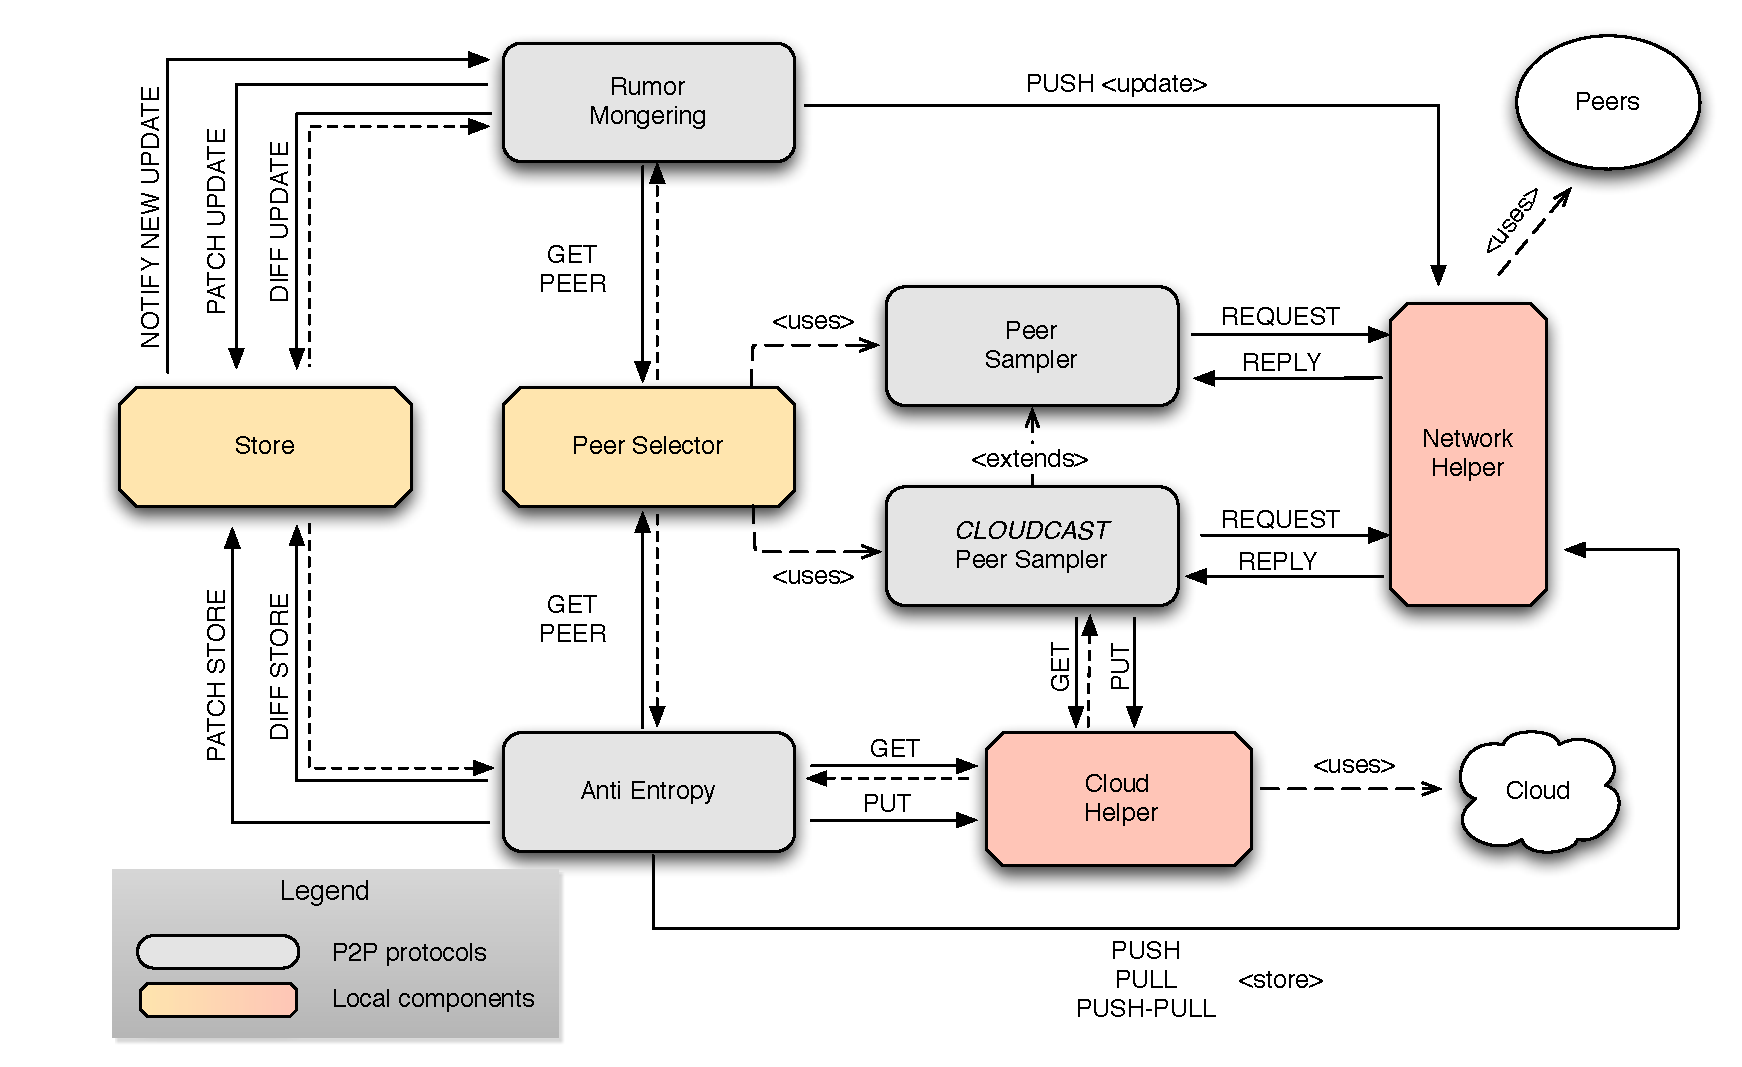
\includegraphics[width=\textwidth]{cloudypeer-architecture.pdf}
  \caption{Architectural overview of \cloudypeer}
  \label{fig:cloudypeer-sequence-architecture}
\end{figure}

\begin{figure}[H]
  \centering
  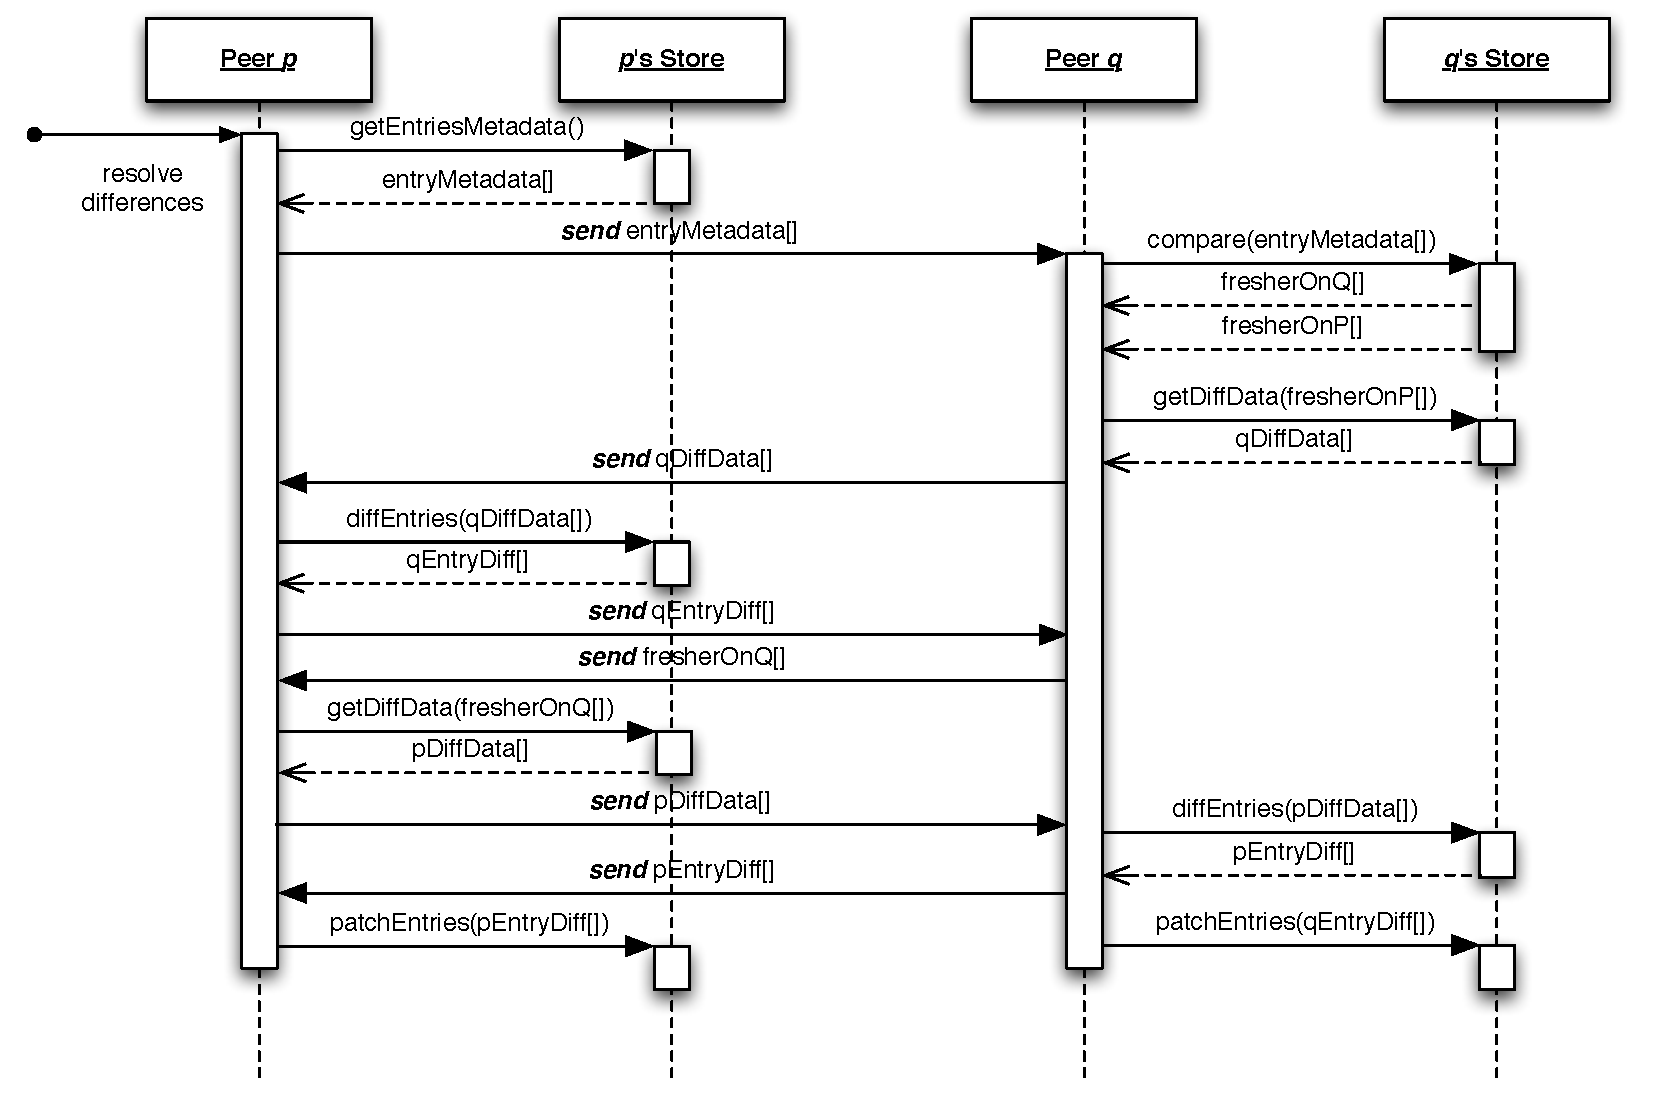
\includegraphics[width=\textwidth]{cloudypeer-antientropy-peer.pdf}
  \caption{Sequence diagram of an \antientropy\ cycle involving a remote
    peer (\PUSHPULL\ strategy)}
  \label{fig:cloudypeer-sequence-antientropy-peer}
\end{figure}

\begin{figure}[H]
  \centering
  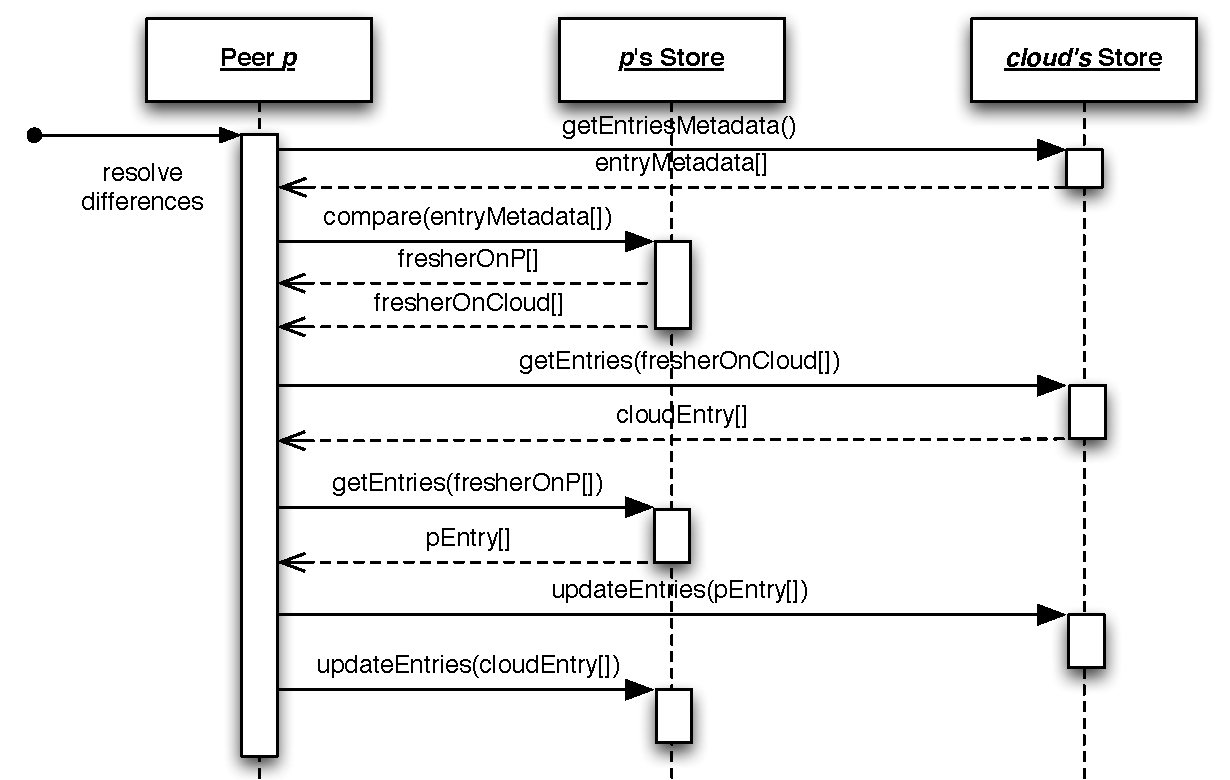
\includegraphics[width=\textwidth]{cloudypeer-antientropy-cloud.pdf}
  \caption{Sequence diagram of an \antientropy\ cycle involving the
    \cloud\ (\PUSHPULL\ strategy)}
  \label{fig:cloudypeer-sequence-antientropy-cloud}
\end{figure}


\begin{figure}[H]
  \centering
  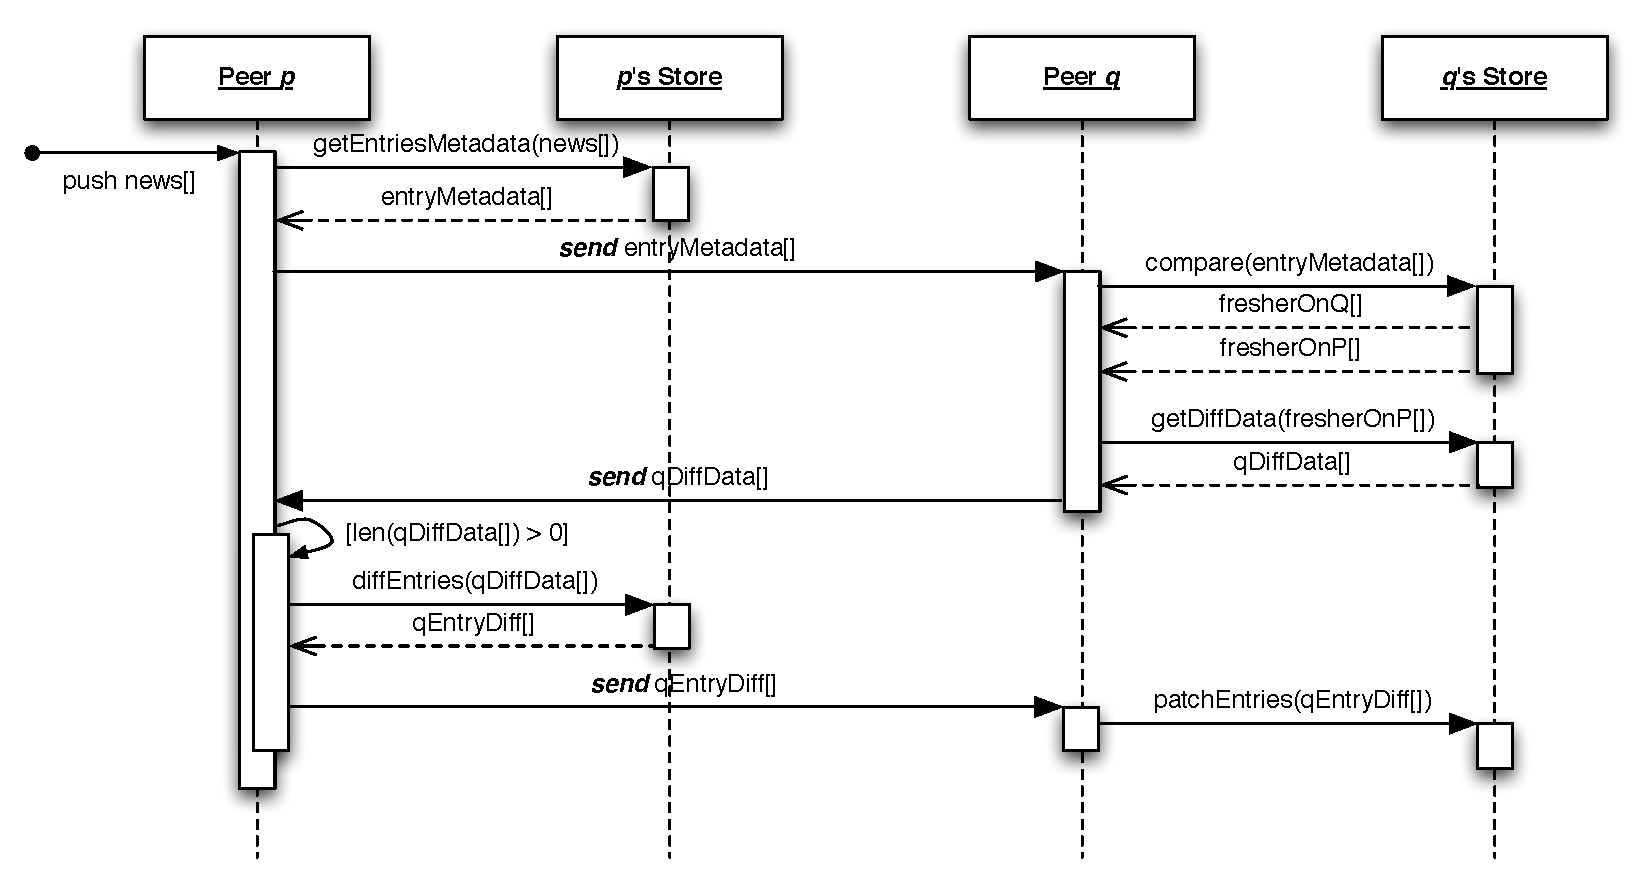
\includegraphics[width=\textwidth]{cloudypeer-rumormongering.pdf}
  \caption{Sequence diagram of a \rumormongering\ cycle}
  \label{fig:cloudypeer-sequence-rumormongering}
\end{figure}

\begin{figure}[H]
  \centering
  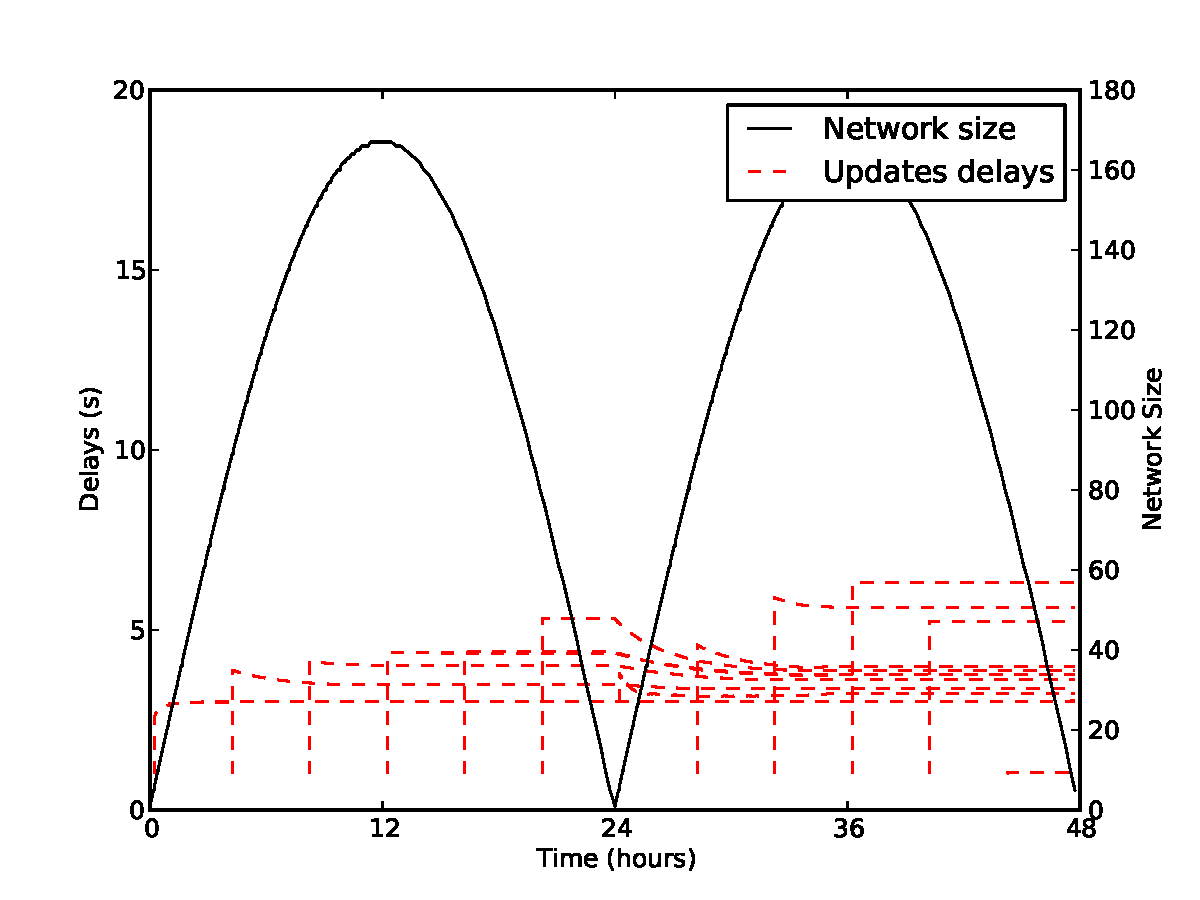
\includegraphics[width=\textwidth]{cloudypeer-oscillating-delays.pdf}
  \caption{Progressive delays in a dynamic scenario}
  \label{fig:cloudypeer-oscillating-delays}
\end{figure}
